\documentclass{article}
\usepackage[utf8]{inputenc}

\usepackage[T2A]{fontenc}
\usepackage[utf8]{inputenc}
\usepackage[russian]{babel}

\usepackage{amsmath}
\usepackage{graphicx}

\title{Вычислительная техника}
\author{Лисид Лаконский}
\date{October 2022}

\begin{document}

\maketitle
\tableofcontents
\pagebreak

\section{Вычислительная техника - 17.10.2022}

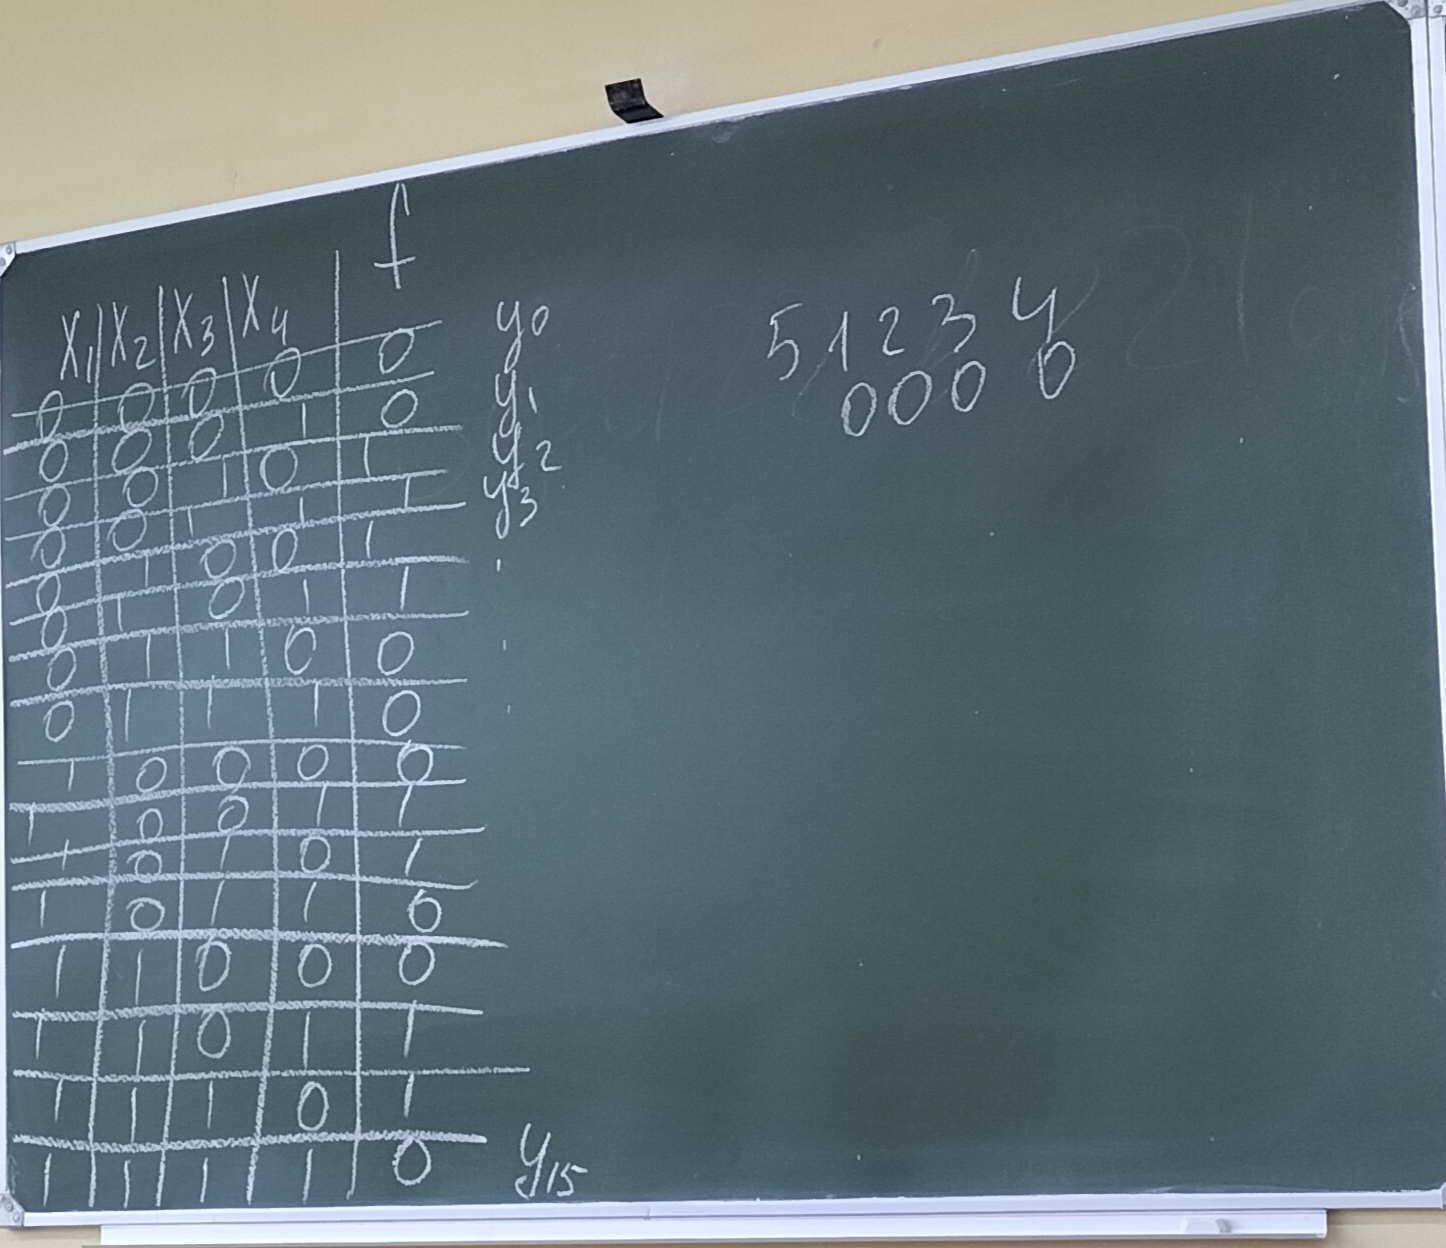
\includegraphics[width=\textwidth]{assets/image_1.jpg}

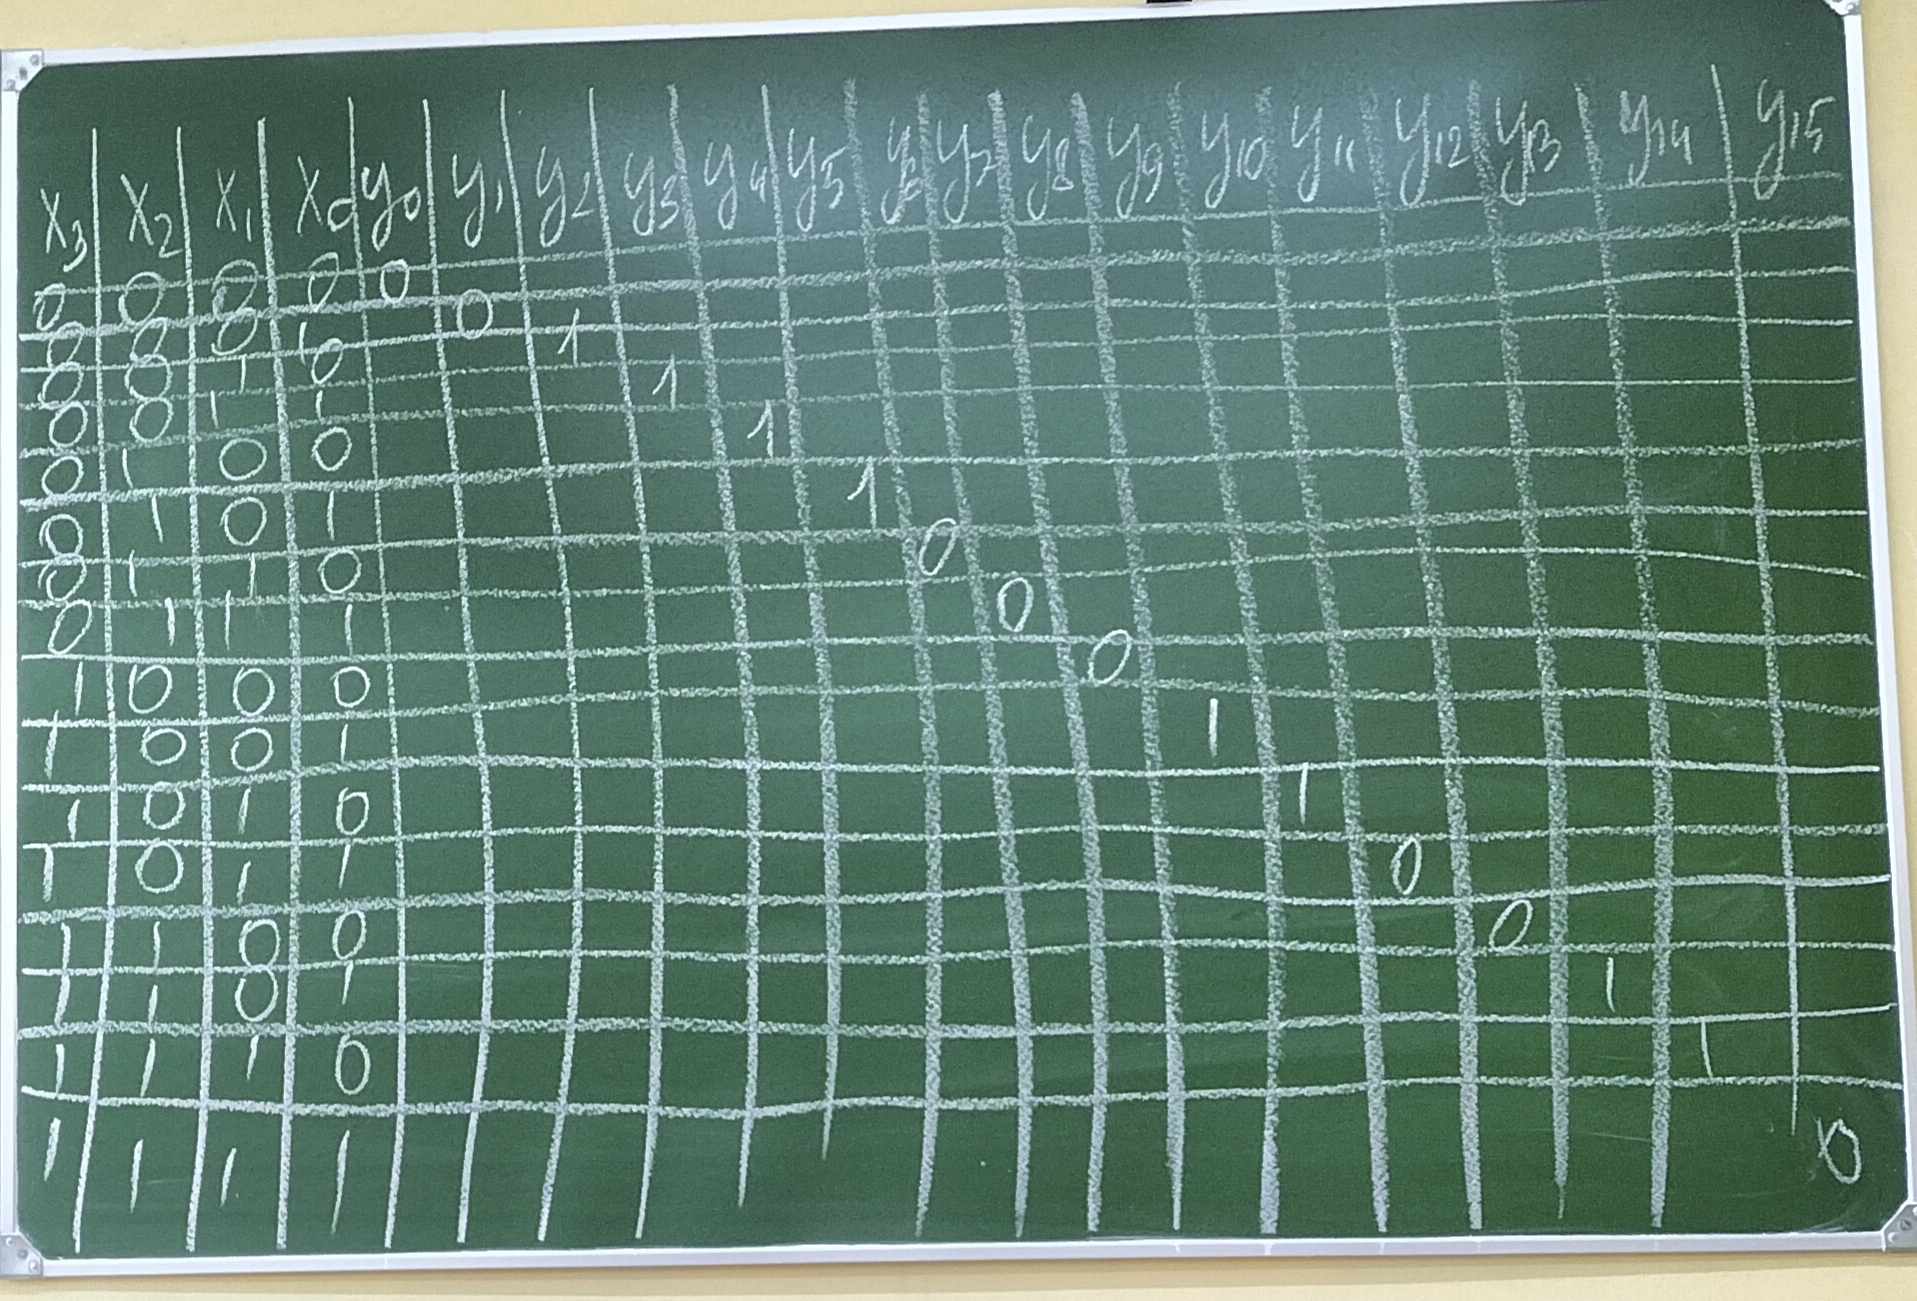
\includegraphics[width=\textwidth]{assets/image_2.jpg}

Показать работоспособность - попереключать ключики - показать, что лампчка зажигается.

\end{document}